\documentclass[11pt,a4paper]{article}
\usepackage[margin=22mm]{geometry}
\usepackage[T1]{fontenc}
\usepackage{lmodern,amsmath,amssymb,booktabs,longtable,graphicx,microtype,array}
\usepackage{enumitem,float}
\usepackage[hidelinks]{hyperref}
\usepackage{fancyhdr}
\setlist{nosep,leftmargin=*}
\setlength{\parindent}{0pt}
\setlength{\parskip}{4pt}
\setlength{\emergencystretch}{2em}
\setlength{\headheight}{14pt}
\pagestyle{fancy}\fancyhf{}\lhead{Tree-Type Neural Networks}\rhead{2025EEA3026}\cfoot{\thepage}
\newcommand{\ind}{\mathbf{1}}
\begin{document}
\hypersetup{pageanchor=false}
\begin{titlepage}
\thispagestyle{empty}
\centering
{\Large \textbf{ASSIGNMENT 4}}\\[2cm]
{\large \textbf{MACHINE LEARNING AND OPTIMIZATION (ELL7285)}}\\[1cm]
{\Large \textbf{TREE-TYPE NEURAL NETWORKS}}\\[0.4cm]
{\large Neural correction nodes, interpolation and compression\\on CIFAR-10 and Cats vs Dogs}\\[2cm]

\textbf{Submitted by}\\[0.5cm]
{\large Durgesh Singh (2025EEA3026)}\\[2cm]

\textbf{Under the guidance of}\\[0.2cm]
{\large Prof. Jayadeva}\\[2cm]

\textit{In partial fulfilment of the requirements for the award of the degree of}\\[0.3cm]
\textbf{Master of Technology}\\[1.5cm]

\IfFileExists{iitd_logo.png}{
\includegraphics[width=0.25\linewidth]{iitd_logo.png}\\[1cm]}{\vspace{2cm}}
Department of Electrical Engineering\\[0.2cm]
\textbf{Indian Institute of Technology Delhi}\\[0.5cm]
\textbf{October 2026}
\end{titlepage}
\hypersetup{pageanchor=true}
\begin{abstract}
This assignment implements the correction-tree construction from the class notes using small neural networks at every learned node. A frozen ImageNet-pretrained MobileNetV3-Small supplies a shared 576-dimensional representation. Children learn the false-negative and false-positive correction tasks of their parent; a constrained logistic output refit combines their decisions. Across three training seeds, trees with hidden width 16 on CIFAR-10 and width 8 on Cats vs Dogs achieve zero training errors on 45,000 and 17,476 images, respectively. Greedy pruning retains perfect training fit and reduces these models to 11--12 nodes and two nodes. Their mean test accuracies are 88.09\% and 97.52\%; a two-node width-16 Cats vs Dogs model reaches 97.85\%. Wider root-only CIFAR-10 networks generalize better. With clean labels the width sweeps show a validation-log-loss peak near interpolation but no peak in classification error. With 15\% training-label noise, double descent appears in test error: CIFAR-10 shows the complete classical curve (14.7\% at width 8, 33.8\% at width 64, 19.5\% at width 1024), and Cats vs Dogs and the correction trees on both datasets show the interpolation peak followed by descent. Under noise, most of the children's targets (76--89\% below the interpolation threshold) are flipped labels, so the corrections memorize noise; validation-based pruning removes them and restores the root's test error. Node visualizations, root-refitting controls and exact prediction-skipping bounds clarify what the branches contribute and what they do not.
\end{abstract}
\textbf{GitHub repository:} \url{https://github.com/dugu01/Tree_Network_Revisited_2025EEA3026}

\section{Question, approach and relation to the earlier assignment}
The earlier assignment asked for a generic optimization formulation of a tree whose nodes can themselves be classifiers. The present task additionally requires neural nodes, near-perfect image-training accuracy, a search for double descent, receptive-field visualizations and size reduction. The structure used here follows the supplied class note \cite{class}: children \emph{correct a parent's decisions}. It is not a conventional decision tree that sends each image down exactly one path.

The earlier supplied implementation defaulted to linear SVM nodes and heuristic correction weights. This implementation uses one-hidden-layer MLP nodes, a constrained output-layer optimization and an explicit acceptance check. Historical results in the previous submission are not treated as newly reproduced measurements. The present CIFAR-10 result also benefits from external ImageNet supervision, so it is not a controlled accuracy comparison with that earlier system.

The practical choice was to spend image-processing effort once, cache the features, and study many inexpensive correction heads on an 8-GB M3 Mac. This makes the architecture and capacity study feasible without a large GPU. The investigation separates four questions: can branches remove residual training errors; do they improve held-out predictions; which branches remain necessary after fitting; and does increasing capacity produce the expected double-descent shape?

\section{Architecture and optimization}
\subsection{Shared features and small neural nodes}
The encoder is the feature stack and global average pool of MobileNetV3-Small \cite{mobilepaper,mobile}, with its ImageNet classifier removed. It contains 927,008 frozen parameters. Official pretrained transforms resize to 256 pixels and centre-crop to $224\times224$, then apply ImageNet normalization. Upsampling CIFAR-10 does not recover missing detail. Cached vectors $z=\phi(x)\in\mathbb{R}^{576}$ are standardized by the training mean and standard deviation only; each standard deviation is floored at $10^{-5}$.

At node $v$, with hidden width $h$,
\begin{align}
 r_v(z)&=\operatorname{ReLU}(W_vz+c_v), & s_v(z)&=u_v^\top r_v(z)+b_v,\\
 F_v(z)&=s_v(z)+a_v H_A(z)-d_v H_B(z), & H_v(z)&=\ind[F_v(z)\geq0],\quad a_v,d_v\geq0.
\end{align}
An absent child contributes zero. Child decisions are themselves recursively corrected binary outputs. A node MLP has
\begin{equation}
P_{\mathrm{node}}=576h+h+h+1=578h+1
\end{equation}
parameters; each retained child connection adds one correction scalar. The count includes the trunk once, even though it is frozen. It excludes non-parameter buffers and Python/checkpoint overhead, so parameter reduction is not a direct measurement of file-size reduction.

Cats vs Dogs uses one tree, with dog as class one. CIFAR-10 uses ten one-versus-rest (OVR) trees sharing the trunk and predicts $\arg\max_k F_k(z)$. Thus the multiclass implementation is a forest of correction trees. Correct binary classification for all OVR tasks is sufficient for a correct argmax, but is not necessary. A few local binary mistakes can coexist with zero multiclass training errors.

\subsection{Targets inherited by the children}
For each node's local labels $y_i\in\{0,1\}$, construct groups using its initial MLP prediction $\ind[s_v(z_i)\geq0]$:
\begin{center}
\begin{tabular}{ccccc}\toprule
Group & Parent prediction & Desired label & Child $A$ target & Child $B$ target\\\midrule
$C_1$ & 0 & 0 & 0 & don't care\\
$C_2$ & 1 & 1 & don't care & 0\\
$C_3$ & 0 & 1 & 1 & 0\\
$C_4$ & 1 & 0 & 0 & 1\\\bottomrule
\end{tabular}
\end{center}
$A$ repairs false negatives and excludes $C_2$ from its training set; $B$ repairs false positives and excludes $C_1$. Keeping the other groups teaches when a correction must remain inactive. Training children only on mistakes would omit this information. Growth stops at depth two, counting a root as depth zero, or when there are no errors or too few local examples. Single-class local targets use a constant decision.

\subsection{Training and the constrained readout problem}
Each MLP is trained by Adam on class-balanced binary cross-entropy (BCE). A class-$c$ example has weight $N/(2N_c)$. The final sweeps use learning rate $10^{-3}$, batch size 512, 100 epochs per learned node, no dropout or weight decay, and no stochastic image augmentation. These choices deliberately permit memorization. The shared encoder is never fine-tuned.

Once children are trained, freeze the parent's hidden activations and child decisions. Refit the parent's output coefficients by
\begin{align}
\min_{u,b,a,d}\quad &\frac1N\sum_{i=1}^{N}\left[\log(1+e^{f_i})-y_if_i\right]
 +\frac{\lambda}{2}\bigl(\|u\|_2^2+a^2+d^2\bigr),\label{eq:refit}\\
\text{subject to}\quad &f_i=u^\top r_i+b+aH_A(z_i)-dH_B(z_i),\qquad a,d\geq0.
\end{align}
Here $\lambda=10^{-6}$; the bias is unregularized. This refit uses unweighted BCE, unlike the initial balanced MLP training. With fixed $r_i,H_A,H_B$, $f_i$ is affine in the unknowns and the logistic loss has second derivative $\sigma(f_i)(1-\sigma(f_i))\geq0$. The Hessian is a positive-semidefinite weighted Gram matrix plus the regularizer. Therefore this subproblem is convex on its feasible set. Representation learning and adaptive tree growth remain nonconvex.

The code uses numerically stable logistic loss, analytic gradients and L-BFGS-B, with a 120-iteration cap; convergence information is recorded. A candidate is accepted only if its pair (number of training mistakes, unweighted BCE) is lexicographically better than the original parent. Rejected candidates lose their proposed children. A further float32 check prevents a rounding-induced increase in local error. This guarantees non-increase of accepted \emph{local error counts}; it does not guarantee preservation of every previously correct sample, improvement of multiclass argmax, or generalization.

The class-note margin formulation can use $t_iF_i\geq1-q_i$, $q_i\geq0$, where $t_i=2y_i-1$. A positive $q_i$ signals a margin violation, which need not be a classification error. Equation~\eqref{eq:refit} is the smooth surrogate actually implemented; no claim is made that the code solves the original full mixed discrete/continuous margin problem globally.

\section{Data, protocol and implementation checks}
\begin{center}
\begin{tabular}{lrrr}\toprule
Dataset & Training & Validation & Test\\\midrule
CIFAR-10 & 45,000 & 5,000 & 10,000\\
Cats vs Dogs, cleaned & 17,476 & 3,745 & 3,745\\\bottomrule
\end{tabular}
\end{center}
CIFAR-10 uses its official test set; 10\% of the official training set forms a stratified validation split \cite{cifar}. Cats vs Dogs uses the Microsoft PetImages archive \cite{cats}. Of 25,000 image files, two were unreadable, 26 were redundant same-label copies, and six belonged to two exact-pixel groups with conflicting labels. Every member of a conflicting group was excluded, before splitting. The remaining 24,966 images were stratified 70/15/15. Training contains 8,736 cats and 8,740 dogs; validation and test each contain 1,872 cats and 1,873 dogs. Exact RGB-pixel hashes include image dimensions. This does not detect near-duplicates or establish absence of overlap with ImageNet.

The initial loader correctly detected conflicting labels but aborted preparation. It was revised to exclude entire ambiguous groups, record the reason for every excluded file, and preserve the original images. The final cleaning policy is included in cache metadata. The common split seed is 17; optimization seeds are 17, 29 and 43. There is one fixed split per dataset, so seed standard deviations measure optimization variability, not uncertainty over independent data splits.

The CIFAR-10 sweep uses widths $2,4,8,16,32,64,128,256$; Cats vs Dogs uses $1,2,4,8,16,32,64,128$. This gives 48 width--seed configurations and 96 initial root/tree fits. Early stopping at zero errors is disabled in sweeps; ordinary pilot/main commands can stop early. Maximum depth, preprocessing and per-node epoch budget are fixed, but topology and total optimization work vary with width. The final comparison also includes a \emph{root + refit} control: retain the original root hidden layer and solve the same readout problem without children. This distinguishes branch effects from better output-layer optimization.

A protocol chosen from training/validation results fixes 12 runs before final test evaluation: all three seeds for CIFAR-10 width 16 and Cats vs Dogs widths 8 and 16; seed 17 for CIFAR-10 widths 64 and 256 and Cats vs Dogs width 32. In each run, root, refitted root, tree and pruned variants receive test evaluation. Within-run validation selection is separately recorded (highest accuracy, then smallest parameter count); it can legitimately select a root-only model. The named tree comparisons below are prespecified scientific comparisons, not retrospectively selected test winners. Test scores were not used for another tuning round. Test features had already been cached; they did not fit the standardizer or the heads.

The Mac records report MPS feature extraction and CPU head fitting with four threads. Main extraction took 109.44 seconds for CIFAR-10 and 79.04 seconds for Cats vs Dogs, excluding download/cleaning. Python 3.11.17, PyTorch 2.14.1 and torchvision 0.29.1 are recorded in the run metadata. Cached-feature timings are not end-to-end image latency measurements.

Validation includes 14 unit tests covering correction targets, refitting, forward agreement, pruning, certified predictions and data cleaning. An exported audit checks reloaded local checkpoints against the recorded training and validation errors. All 472,268 exported prediction rows across 15 audits were checked for internal consistency, and all 48 final test records agree with their confusion-matrix totals. The image checkpoints themselves were not re-run while preparing this report, so this is a consistency check of the saved evidence rather than a new measurement.

\section{Results: interpolation, generalization and controls}\label{sec:results}
\begin{table}[H]\centering\small
\caption{Main controlled comparisons. Accuracy is mean $\pm$ sample SD in percent over seeds 17, 29 and 43. Training errors are the observed range across seeds. CIFAR-10 test size is 10,000; Cats vs Dogs test size is 3,745.}
\begin{tabular}{lllrcc}\toprule
Dataset & Width & Model & Train errors & Validation (\%) & Test (\%)\\\midrule
CIFAR-10 & 16 & Root & 1--3 & 89.49 $\pm$ 0.03 & 88.31 $\pm$ 0.16 \\
CIFAR-10 & 16 & Root + refit & 1--2 & 89.25 $\pm$ 0.14 & 88.30 $\pm$ 0.18 \\
CIFAR-10 & 16 & Tree & 0 & 88.97 $\pm$ 0.14 & 88.10 $\pm$ 0.09 \\
CIFAR-10 & 16 & Pruned & 0 & 88.97 $\pm$ 0.14 & 88.09 $\pm$ 0.09 \\
Cats/Dogs & 8 & Root & 3--8 & 97.69 $\pm$ 0.06 & 97.59 $\pm$ 0.20 \\
Cats/Dogs & 8 & Root + refit & 3--8 & 97.72 $\pm$ 0.07 & 97.59 $\pm$ 0.20 \\
Cats/Dogs & 8 & Tree & 0 & 97.66 $\pm$ 0.18 & 97.52 $\pm$ 0.15 \\
Cats/Dogs & 8 & Pruned & 0 & 97.66 $\pm$ 0.18 & 97.52 $\pm$ 0.15 \\
Cats/Dogs & 16 & Root & 1--4 & 97.91 $\pm$ 0.09 & 97.82 $\pm$ 0.04 \\
Cats/Dogs & 16 & Root + refit & 1--4 & 97.91 $\pm$ 0.04 & 97.79 $\pm$ 0.06 \\
Cats/Dogs & 16 & Tree & 0 & 97.89 $\pm$ 0.07 & 97.85 $\pm$ 0.13 \\
Cats/Dogs & 16 & Pruned & 0 & 97.89 $\pm$ 0.07 & 97.85 $\pm$ 0.13 \\
\bottomrule

\end{tabular}\label{tab:main}
\end{table}
The first tested width at which the \emph{tree} interpolates for every seed is 16 for CIFAR-10 and 8 for Cats vs Dogs. The root-only width-16 CIFAR models leave 1, 1 and 3 multiclass errors; their trees remove all of them. Root refitting alone leaves 1, 1 and 2. Similarly, Cats vs Dogs width-8 roots and refitted roots leave 5, 8 and 3 errors, while all trees fit perfectly. This supports a specific conclusion: these correction branches resolve residual training errors not removed by the chosen root-only refit. It does not show that no alternative optimizer could fit the smaller root.

The held-out results give a different answer. CIFAR-10 width-16 trees average 88.10\% test accuracy versus 88.31\% for the corresponding roots. Cats vs Dogs width-8 trees average 97.52\% versus 97.59\% for the roots. The width-16 Cats vs Dogs trees average 97.85\%, a small increase over the roots' 97.82\%, with no strong superiority claim from three seeds. Exact interpolation is achieved, but fitting the final training exceptions need not improve generalization.

For context, the prespecified seed-17 CIFAR root-only width-64 and width-256 models obtain 89.97\% and 90.29\% test accuracy, respectively. Their head sizes are 369,930 and 1,479,690 parameters. The width-256 root + refit obtains 90.30\%, but has lower validation accuracy than the original root; the 0.01-point test difference is not used to change selection. The seed-17 Cats vs Dogs width-32 root has 18,497 head parameters, zero training errors and 97.76\% test accuracy. Its refitted counterpart was the within-run validation winner but obtains 97.65\% on test. These cases illustrate why selection must precede test inspection.

The earlier 2,000-image CIFAR pilot also reached interpolation, and its 25-node tree pruned to ten roots. However, a refitted root-only control already interpolated that pilot. Consequently, the pilot does not establish that branches were necessary. The larger controlled experiments provide the stronger evidence reported here.

\section{Capacity curves and the double-descent question}\label{sec:capacity}
\begin{figure}[H]\centering
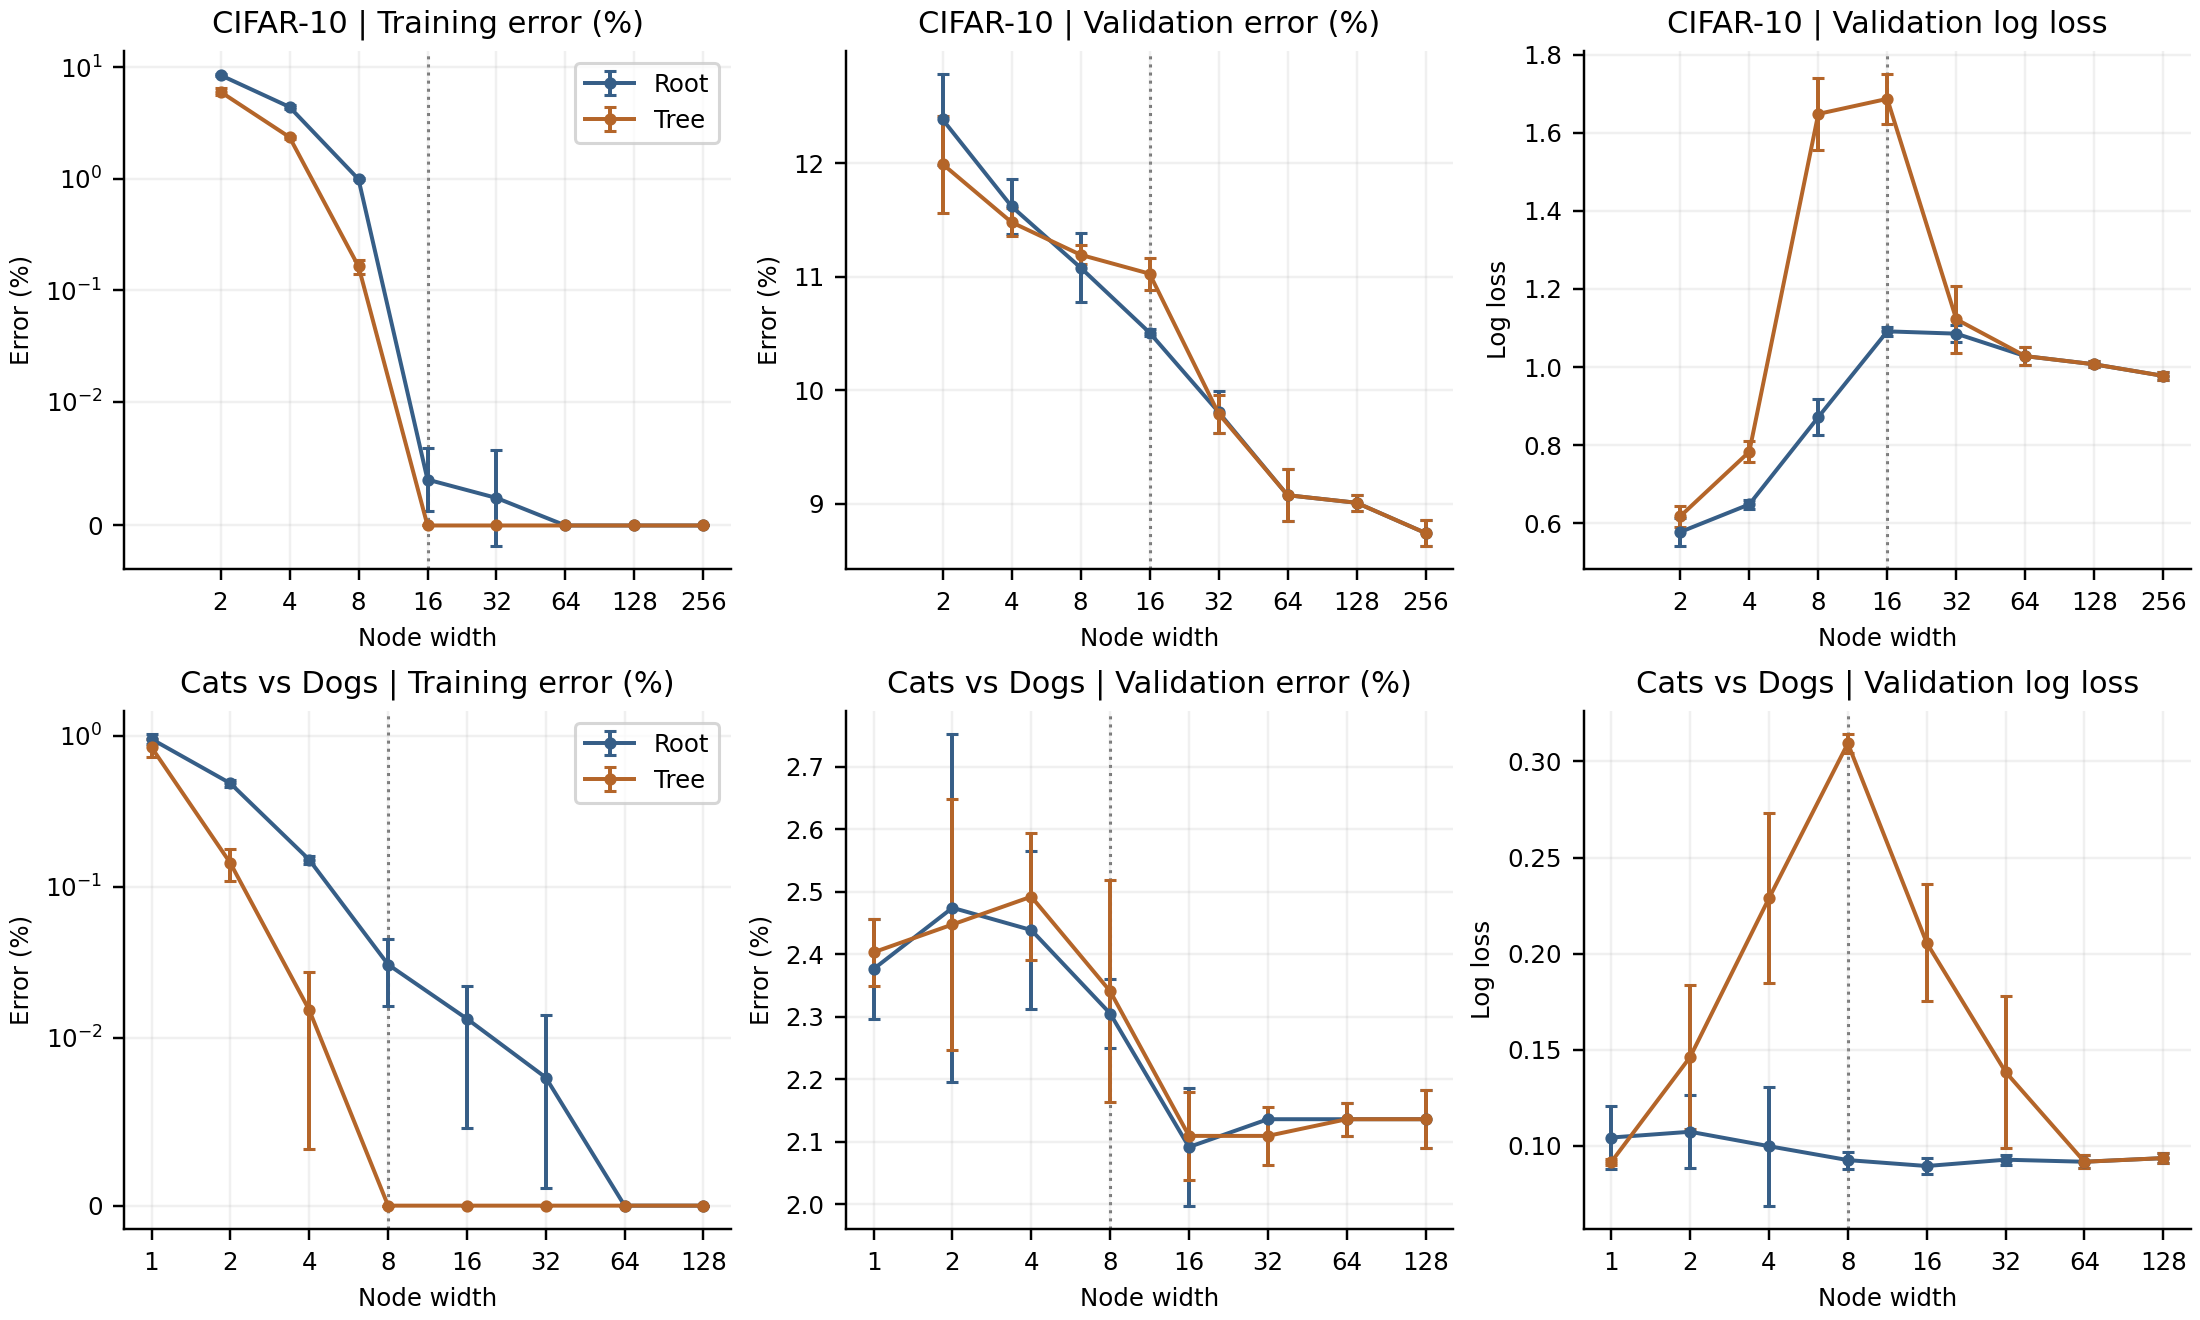
\includegraphics[width=\linewidth]{figures/capacity_curves.png}
\caption{Width sweeps on the fixed main splits. Points and bars show means and sample SD over three seeds. The dotted line marks the first tested tree width with zero training errors in all seeds (16 for CIFAR-10, 8 for Cats vs Dogs). Training error uses a symmetric-log scale to display small nonzero errors and exact zero. These are validation curves; test scores did not choose widths.}\label{fig:capacity}
\end{figure}
Double descent is a capacity-dependent deterioration near interpolation followed by renewed improvement beyond it; a complete classical double-descent curve also contains an earlier descent \cite{dd}. Our results do not justify claiming that full pattern in classification error. Mean CIFAR-10 root validation error falls across the tested widths. Mean CIFAR-10 tree validation error also decreases across the tested widths, without an interpolation peak. Cats vs Dogs classification-error differences are small and sensitive to seed.

Log loss provides a more repeatable observation. CIFAR-10 tree validation log loss rises from 0.618 at width 2 to 1.687 at width 16, then falls to 0.977 at width 256. Cats vs Dogs rises from 0.092 at width 1 to 0.309 at width 8, then falls to about 0.092 at width 64. Peaks occur near the observed tree interpolation widths, and the decline persists across seeds. The appropriate description is \emph{an interpolation-associated validation-loss peak with post-interpolation descent}, rather than an established complete double-descent result.

Classification accuracy depends on decision ordering or sign, whereas log loss penalizes confident mistakes. Output refitting can increase score magnitudes substantially while barely changing labels. For example, CIFAR-10 width-16 mean test log loss is 1.220 for roots, 2.056 for refitted roots and 1.863 for trees. The corresponding accuracies differ much less. Cats vs Dogs width-8 refitting leaves the test error count unchanged in every seed, but mean test log loss increases from 0.095 to 0.243. This supports concern about confidence, not a calibrated-probability claim. CIFAR log loss uses a softmax over independently trained OVR scores, which are not jointly calibrated.

\begin{figure}[H]\centering
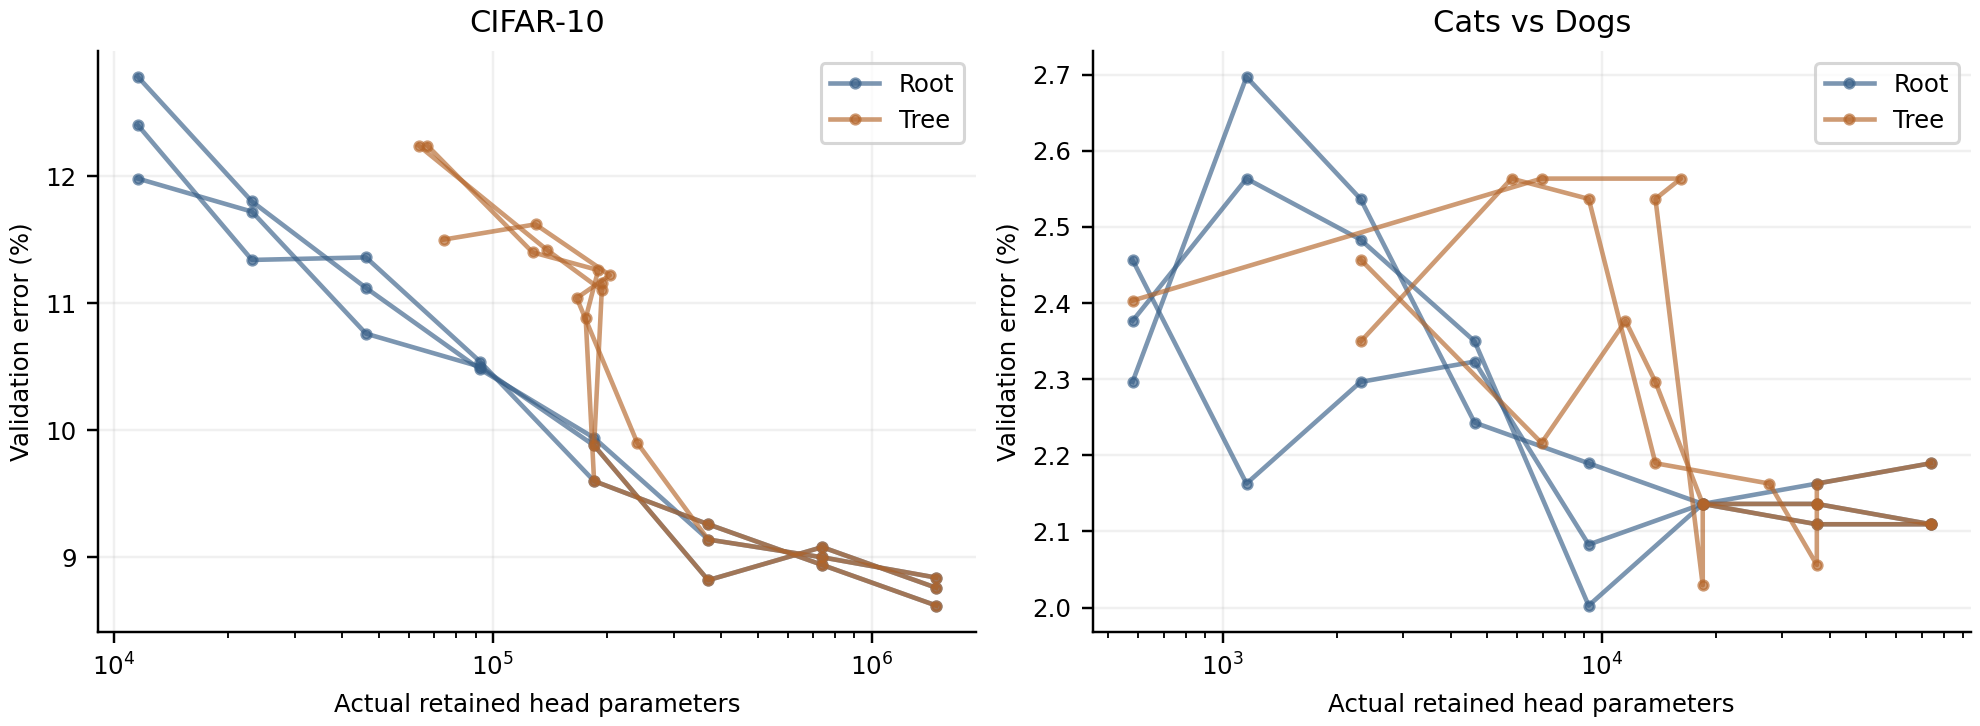
\includegraphics[width=.96\linewidth]{figures/parameter_curves.png}
\caption{The same validation classification errors against retained head parameters. Each thin curve is one seed, connected in increasing-width order. Adaptive growth makes parameter count nonmonotonic; a larger node can produce a smaller tree. The frozen trunk adds 927,008 parameters to every point.}\label{fig:parameters}
\end{figure}
At seed 17, moving CIFAR-10 width 8 to width 16 reduces the head from 203,534 to 166,490 parameters because node count falls from 44 to 18. Cats vs Dogs width 4 to width 8 similarly reduces the head from 16,197 to 13,877. Therefore width alone is not an ordered measure of realized tree complexity. A fixed-topology or explicitly parameter-budgeted study would be needed to separate this effect from classic width-based double descent. Epoch-wise behaviour and the effect of label noise are examined separately in Section~\ref{sec:noise}.

\section{Label noise: double descent and what the corrections learn}\label{sec:noise}
With clean labels the capacity sweeps show a log-loss peak but no peak in classification error (Section~\ref{sec:capacity}). The classical test-error peak appears when a model is only just able to memorize \emph{wrong} labels \cite{dd}, so this section repeats the capacity study with corrupted training labels, for both datasets and for the correction tree itself. The clean-label results above are unchanged.

\subsection{Design}
On the same cached features, 15\% of the training labels are corrupted with a fixed noise seed shared by every run (Cats vs Dogs: 2,621 of 17,476 labels flipped, approximately 15\%; CIFAR-10: exactly 6,750 of 45,000 moved to a uniformly random other class). Validation and test labels stay clean. Two model families are swept over width, each with optimization seeds 17, 29 and 43:
\begin{itemize}
\item \textbf{Fixed-topology root-only networks} (\texttt{extras/label\_noise\_double\_descent.py}). For Cats vs Dogs this is exactly the root-node model (one hidden ReLU layer, $578h+1$ parameters, class-balanced BCE). For CIFAR-10 a single softmax MLP ($587h+10$ parameters) replaces the ten one-vs-rest roots to keep the dense sweep tractable. Adam (learning rate $10^{-3}$, batch 512), no weight decay, 300 epochs without early stopping. Each noisy sweep has a matched clean-label control; Cats vs Dogs is repeated for two further noise draws and has an epoch-wise run (width 16, 1000 epochs).
\item \textbf{The correction tree} (\texttt{extras/label\_noise\_tree.py}), using the unchanged \texttt{tree\_model.py} with the main-sweep settings (depth 2, 100 epochs per node, constrained refit). For each width and seed it records the root-only model (whose hidden layer was checked to be identical to the tree's root), the tree, the tree pruned by the original rule (no loss of training accuracy, at most 0.5 points of validation accuracy), and the tree pruned by a \emph{validation-only} rule (a child is kept only if removing it lowers validation accuracy).
\end{itemize}
These are exploratory test curves, reported at every width. No model from this study enters the clean-label comparisons, whose fixed evaluation protocol (Section~\ref{sec:protocol}) is unaffected; the width used for the epoch-wise run (16) was chosen after inspecting the width sweep. All runs used the experiment Mac; \texttt{extras/build\_noise\_report.py} checks the records for completeness and regenerates every figure and table here.

\subsection{Double descent appears under label noise}
\begin{figure}[H]\centering
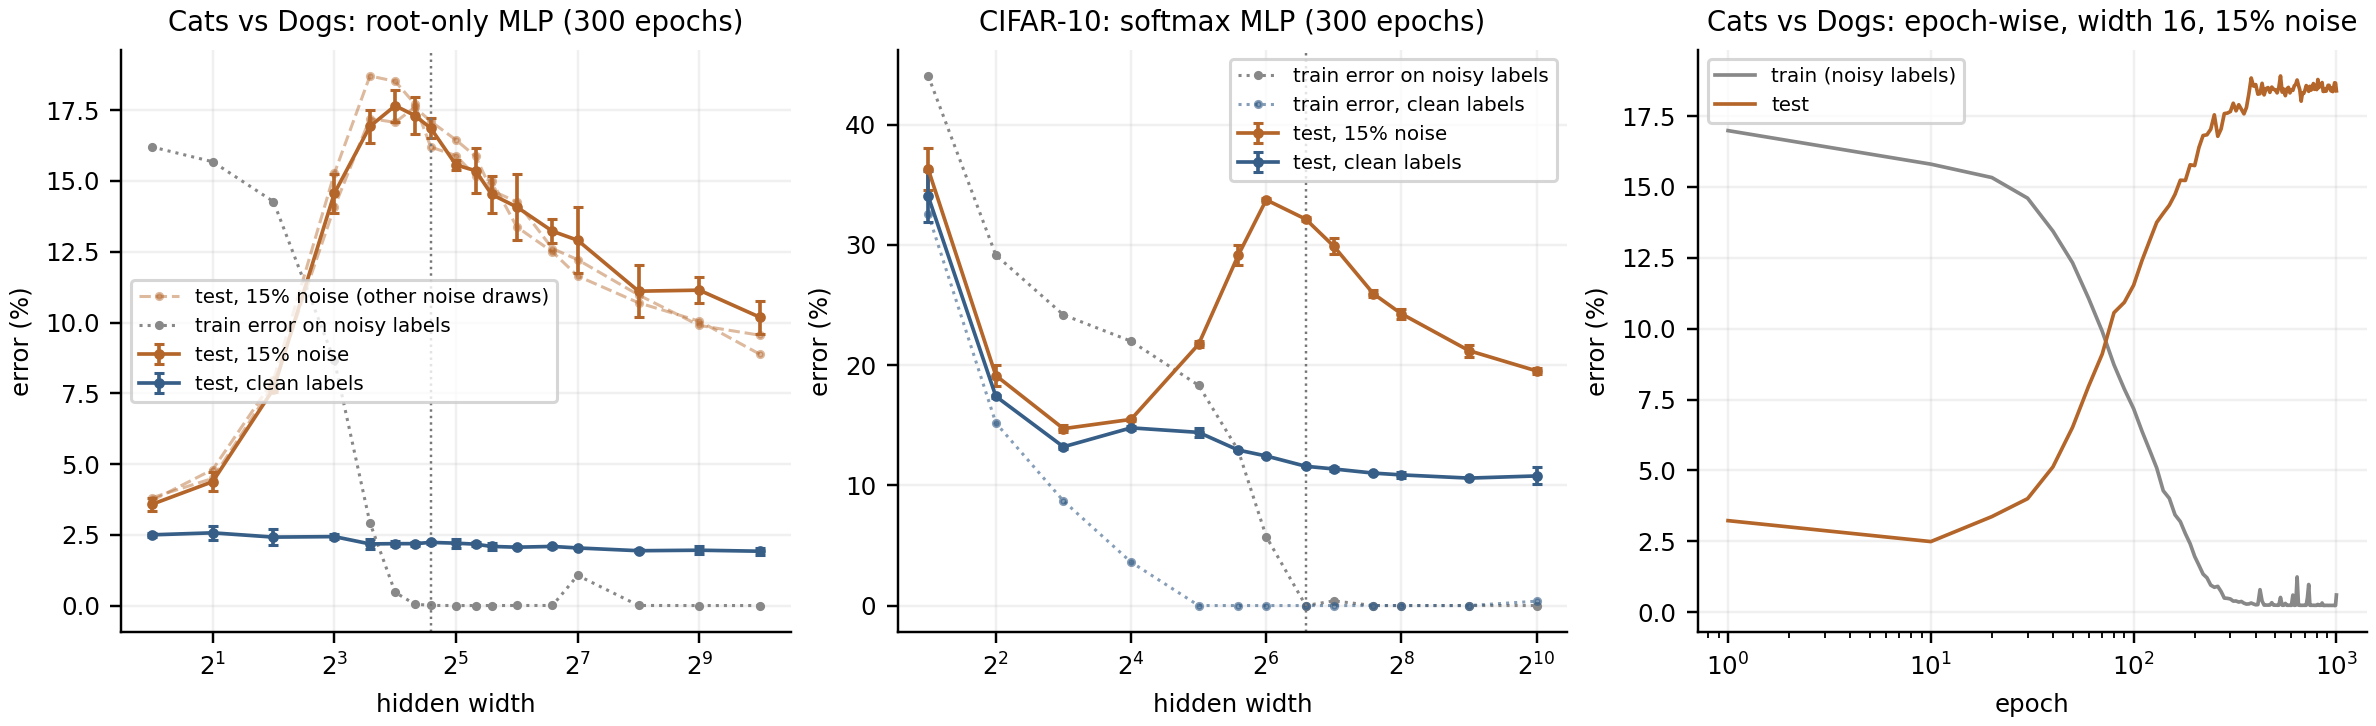
\includegraphics[width=\linewidth]{figures/noise_root_curves.png}
\caption{Fixed-topology root-only networks. Error bars are sample SD over three optimization seeds. Dotted vertical lines mark the first width whose mean noisy-train error is below 0.05\%. Dashed curves (left) are two further noise draws. Right: epoch-wise mean over three seeds.}\label{fig:noiseroot}
\end{figure}
\begin{table}[H]\centering\small
\caption{Root-only width sweeps (mean over three seeds; test SD in parentheses). Bold marks the best width before the peak and the peak.}
\begin{tabular}{lrrrrrr}\toprule
& & & \multicolumn{2}{c}{15\% label noise} & \multicolumn{2}{c}{Clean labels}\\\cmidrule(lr){4-5}\cmidrule(lr){6-7}
Data & Width & Params & Train err.\ (\%) & Test err.\ (\%) & Train err.\ (\%) & Test err.\ (\%)\\\midrule
C/D & 1 & 579 & 16.21 & \textbf{3.58} (0.22) & 0.45 & 2.50 \\
C/D & 4 & 2,313 & 14.27 & 7.65 (0.09) & 0.10 & 2.42 \\
C/D & 8 & 4,625 & 8.67 & 14.56 (0.68) & 0.04 & 2.44 \\
C/D & 12 & 6,937 & 2.93 & 16.93 (0.58) & 0.02 & 2.18 \\
C/D & 16 & 9,249 & 0.47 & \textbf{17.66} (0.57) & 0.01 & 2.19 \\
C/D & 20 & 11,561 & 0.05 & 17.31 (0.65) & 0.00 & 2.19 \\
C/D & 24 & 13,873 & 0.01 & 16.87 (0.36) & 0.00 & 2.23 \\
C/D & 32 & 18,497 & 0.00 & 15.57 (0.16) & 0.00 & 2.21 \\
C/D & 64 & 36,993 & 0.01 & 14.08 (1.16) & 0.00 & 2.06 \\
C/D & 128 & 73,985 & 1.07 & 12.91 (1.17) & 0.00 & 2.04 \\
C/D & 256 & 147,969 & 0.01 & 11.11 (0.92) & 0.00 & 1.94 \\
C/D & 1024 & 591,873 & 0.00 & 10.18 (0.58) & 0.00 & 1.92 \\
\midrule
C10 & 2 & 1,184 & 44.05 & 36.29 (1.74) & 32.55 & 34.03 \\
C10 & 4 & 2,358 & 29.15 & 19.13 (0.89) & 15.19 & 17.40 \\
C10 & 8 & 4,706 & 24.18 & \textbf{14.71} (0.28) & 8.70 & 13.20 \\
C10 & 16 & 9,402 & 21.99 & 15.48 (0.14) & 3.61 & 14.78 \\
C10 & 32 & 18,794 & 18.31 & 21.73 (0.26) & 0.00 & 14.40 \\
C10 & 48 & 28,186 & 12.92 & 29.12 (0.83) & 0.00 & 12.93 \\
C10 & 64 & 37,578 & 5.74 & \textbf{33.75} (0.16) & 0.00 & 12.44 \\
C10 & 96 & 56,362 & 0.00 & 32.14 (0.18) & 0.00 & 11.58 \\
C10 & 128 & 75,146 & 0.39 & 29.88 (0.68) & 0.00 & 11.36 \\
C10 & 256 & 150,282 & 0.00 & 24.27 (0.44) & 0.00 & 10.87 \\
C10 & 512 & 300,554 & 0.00 & 21.20 (0.51) & 0.00 & 10.60 \\
C10 & 1024 & 601,098 & 0.00 & 19.51 (0.27) & 0.36 & 10.78 \\
\bottomrule

\end{tabular}\label{tab:noiseroot}
\end{table}
\textbf{The CIFAR-10 softmax MLP shows the complete decrease--increase--decrease curve} (Figure~\ref{fig:noiseroot}, middle). This result belongs to the single softmax MLP, not to the correction-tree architecture, which is treated in Section~\ref{sec:noisetree}. Test error first falls from 36.3\% to 14.7\% at width 8, then rises to 33.8\% at width 64, where the network fits all but 5.7\% of the noisy labels, and falls again once it interpolates, to 19.5\% at width 1024. The peak sits just before the first width at which every seed fits the noisy labels exactly (width 96, about $5.6\times10^4$ parameters for 45,000 examples), as the double-descent account predicts. The clean control has a small bump at its own interpolation point (13.2\% at width 8, 14.8\% at width 16, then 10.6\% at width 512); noise turns this 1.6-point bump into a 19-point peak.

\textbf{Cats vs Dogs shows the peak and the second descent but not the first descent.} Width 1 is already the best model (3.6\%), because the pretrained features make the task almost linearly separable. Test error then rises to 17.7\% at width 16, where noisy-label fit is nearly complete, and falls to 10.2\% at width 1024. Two other noise draws give the same shape (peaks of 18.7\% and 17.6\%; 8.9\% and 9.6\% at width 1024), while the clean control decreases overall from 2.5\% to 1.9\%, with small reversals but no peak. The noise therefore causes the peak. Epoch-wise, width 16 reaches its best test error (2.5\%) after about 10 epochs and degrades to 18.4\% as it memorizes the flipped labels; no second epoch-wise descent occurs within 1000 epochs.

Overparameterization recovers only part of the damage: the widest noisy models remain far worse than the clean ones (10.2\% versus 1.9\%; 19.5\% versus 10.6\%).

\subsection{The correction tree under noise}\label{sec:noisetree}
\begin{figure}[H]\centering
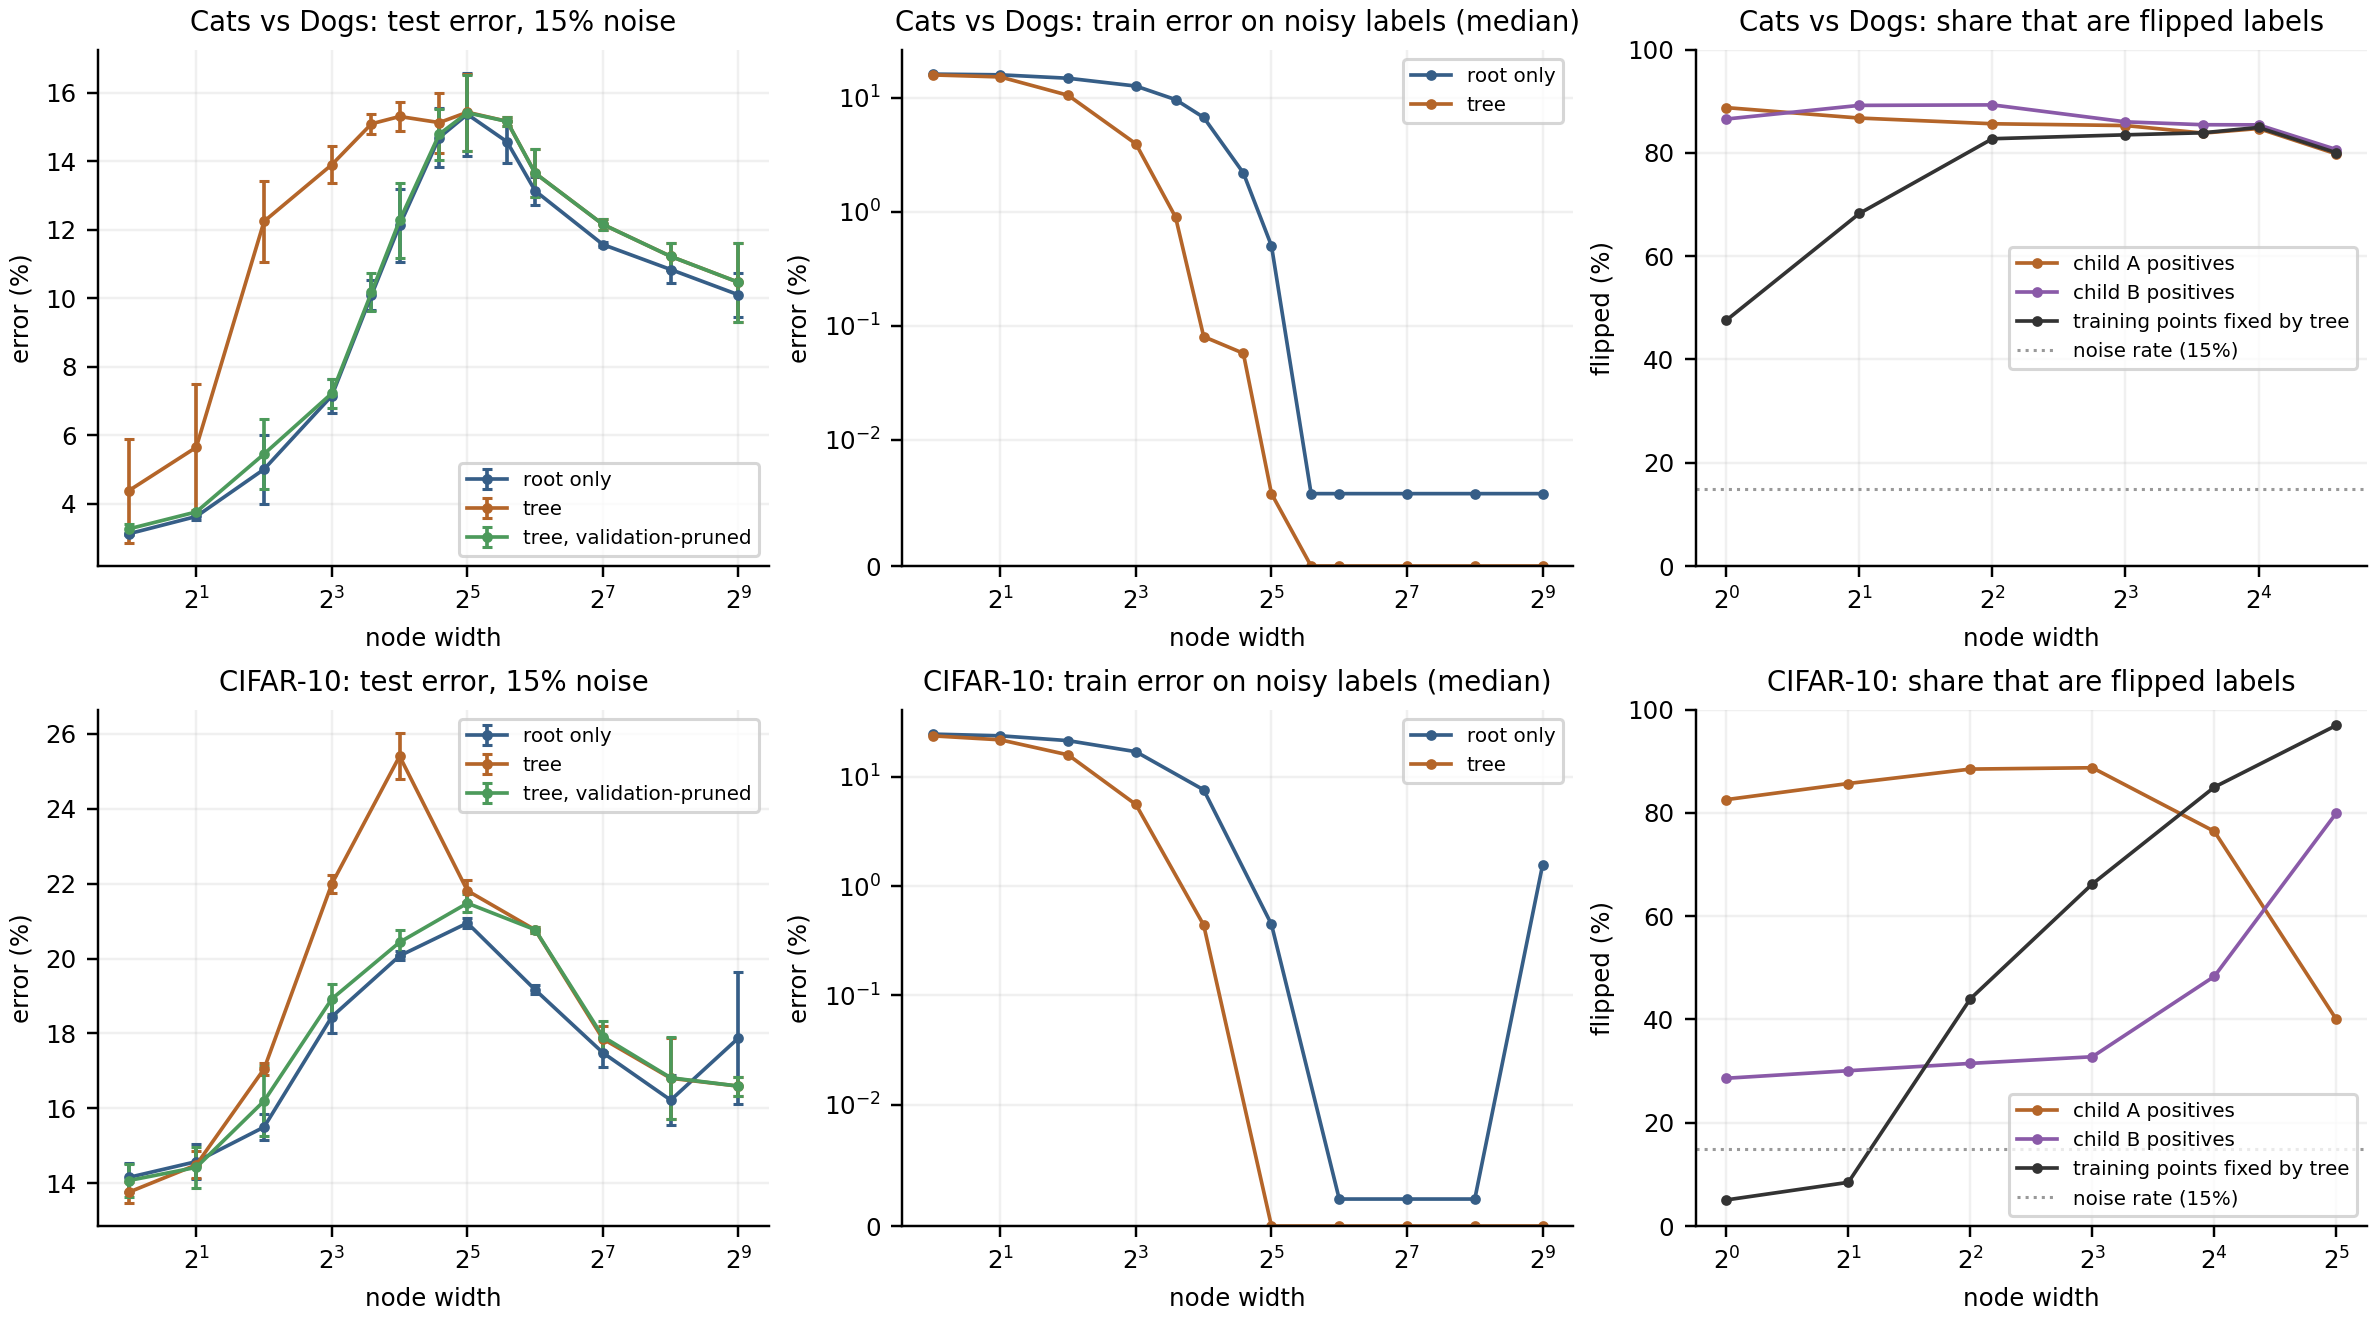
\includegraphics[width=\linewidth]{figures/noise_tree_curves.png}
\caption{Correction trees with 15\% label noise (three seeds). Left: test error of the root-only model, the tree and the validation-pruned tree. Middle: median training error on the noisy labels. Right: share of flipped labels among the positive targets of the roots' children and among the training points the tree fixes, shown only where every root-only run has at least 100 noisy-train errors.}\label{fig:noisetree}
\end{figure}
\begin{table}[H]\centering\small
\caption{Correction trees with 15\% label noise: mean test error (\%) over three seeds, mean noisy-train errors, and the percentage of flipped labels among child-A positive targets / among training points fixed by the tree (``--'' where the root has too few errors to measure).}
\begin{tabular}{lrrrrrrrc}\toprule
Data & Width & Root & Tree & Pruned (orig.) & Pruned (val.) & Root train err. & Tree train err. & Flipped A / fixed\\\midrule
C/D & 1 & 3.12 & 4.38 & 4.41 & 3.27 & 2,833 & 2,775 & 89 / 48 \\
C/D & 4 & 5.01 & 12.25 & 12.07 & 5.46 & 2,599 & 1,861 & 86 / 83 \\
C/D & 8 & 7.16 & 13.90 & 13.90 & 7.23 & 2,238 & 671 & 85 / 83 \\
C/D & 12 & 10.09 & 15.10 & 15.10 & 10.17 & 1,706 & 152 & 84 / 84 \\
C/D & 16 & 12.13 & 15.31 & 15.31 & 12.27 & 1,204 & 17 & 85 / 85 \\
C/D & 24 & 14.70 & 15.13 & 15.13 & 14.79 & 391 & 10 & 80 / 80 \\
C/D & 32 & 15.37 & 15.43 & 15.43 & 15.42 & 74 & 1 & -- \\
C/D & 64 & 13.14 & 13.65 & 13.65 & 13.65 & 1 & 0 & -- \\
C/D & 128 & 11.57 & 12.16 & 12.16 & 12.16 & 1 & 0 & -- \\
C/D & 512 & 10.10 & 10.47 & 10.47 & 10.47 & 1 & 0 & -- \\
\midrule
C10 & 1 & 14.15 & 13.76 & 13.69 & 14.07 & 11,165 & 10,674 & 83 / 5 \\
C10 & 2 & 14.58 & 14.49 & 14.35 & 14.42 & 10,687 & 9,819 & 86 / 8 \\
C10 & 4 & 15.50 & 17.05 & 17.05 & 16.20 & 9,639 & 7,056 & 88 / 44 \\
C10 & 8 & 18.45 & 22.00 & 21.99 & 18.92 & 7,627 & 2,505 & 89 / 66 \\
C10 & 16 & 20.07 & 25.41 & 25.41 & 20.44 & 3,430 & 202 & 76 / 85 \\
C10 & 32 & 20.95 & 21.81 & 21.82 & 21.48 & 195 & 0 & 40 / 97 \\
C10 & 64 & 19.17 & 20.77 & 20.77 & 20.77 & 2 & 0 & -- \\
C10 & 128 & 17.48 & 17.85 & 17.85 & 17.91 & 68 & 0 & -- \\
C10 & 256 & 16.22 & 16.80 & 16.82 & 16.82 & 3 & 0 & -- \\
C10 & 512 & 17.88 & 16.59 & 16.59 & 16.59 & 563 & 0 & -- \\
\bottomrule

\end{tabular}\label{tab:noisetree}
\end{table}
\textbf{The tree also shows a peak followed by descent.} Test error rises from 4.4\% to 15.4\% at width 32 and falls to 10.5\% at width 512 on Cats vs Dogs, and rises from 13.8\% to 25.4\% at width 16 and falls to 16.6\% at width 512 on CIFAR-10. The corrections add capacity: the tree fits the noisy labels at much smaller widths than its own root (CIFAR-10 width 16: about 200 remaining noisy-train errors against 3,430 for the root). On CIFAR-10 the tree's peak therefore moves from width 32 (root-only) to width 16. On Cats vs Dogs both root and tree peak at width 32, but the tree reaches the high-error plateau much earlier (15.1\% at width 12, against 10.1\% for the root). This is consistent with the effective-complexity view of double descent \cite{dd}, in which the peak tracks when the \emph{whole} model can fit the noise.

\textbf{Under noise, the children learn the noise.} Children are trained on their parent's mistakes. When labels are noisy those mistakes are mostly flipped labels: below the interpolation threshold (widths up to 24 on Cats vs Dogs and 16 on CIFAR-10), 76--89\% of child-A positive targets are flipped, against a 15\% noise rate. On Cats vs Dogs, 80--85\% of the training points the tree fixes at widths 4--24 are flipped labels, and the tree is worse than its root at every width (for example 13.9\% against 7.2\% at width 8). CIFAR-10 shows the contrast between helpful and harmful corrections. At widths 1--2 the root underfits the real signal, only 5--8\% of the fixed points are flipped, and the tree is slightly \emph{better} than its root (13.8\% against 14.2\% at width 1). From width 4 onward the fixed points are increasingly flipped labels (44\%, 66\%, 85\%, 97\%) and the tree becomes worse (25.4\% against 20.1\% at width 16). The share of flipped labels among the corrections thus helps explain the observed pattern of when the branches help or hurt; it is a descriptive association across these runs, not a tested predictor.

\textbf{Pruning becomes denoising, but only with a validation criterion.} The original pruning rule forbids any loss of training accuracy, so it keeps the children that memorized noise. Its test error stays close to the tree's, especially around the peak; test counts differ in only 6 of 39 Cats vs Dogs runs and 11 of 30 CIFAR-10 runs, by at most 23 test images, mostly at widths 1--4. The validation-only rule removes them: on Cats vs Dogs all but one of the 39 runs return to the single root node, and test error falls back to the root's level (13.9\% to 7.2\% at width 8; CIFAR-10 width 16: 25.4\% to 20.4\%). Under label noise, minimizing the network and generalizing better therefore coincide, provided the pruning criterion is held-out accuracy rather than training fit. This is consistent with the clean-label finding of Section~\ref{sec:results}: fitting the final training exceptions did not improve test accuracy there either.

\textbf{Two by-products.} First, the child-target groups of Section~\ref{sec:targets} are a promising diagnostic for injected label noise: at width 1 on Cats vs Dogs, 88\% of the root's training errors are flipped labels and they cover 95\% of all flipped labels. This has not been validated as a general noise detector, for example on naturally mislabeled data. Second, the single noisy-train error that wide root-only Cats vs Dogs models keep is one pair of near-identical photographs (\texttt{Dog/9746.jpg} and \texttt{Dog/5733.jpg}, feature distance 0.55 against a median nearest-neighbour distance of 21.2) that the noise gave opposite labels. Exact pixel hashing cannot detect this pair, and the tree fits it with a correction node, which is memorization at its most literal.

\textbf{Caveats.} Six runs ended with unusually many noisy-train errors, consistent with late training instability under Adam without weight decay: Cats vs Dogs root-only width 128 seed 43 (558); CIFAR-10 softmax width 128 seed 29 (520) and clean width 1024 seed 29 (487); and CIFAR-10 tree-sweep root-only width 128 seed 43 (203) and width 512 seeds 29 and 43 (987 and 700). They are kept in all means, which inflates the CIFAR root-only test error at width 512. The CIFAR root-only curve (single softmax MLP, 300 epochs) and the CIFAR tree sweep (ten one-vs-rest roots, 100 epochs per node) differ in architecture and training length, so their peak widths are not directly comparable. One noise rate is studied, the tree and CIFAR-10 sweeps use one noise draw, and the three seeds measure optimization variability only.


\section{Minimizing size and avoiding unnecessary computation}
\subsection{Greedy pruning with fixed constraints}
For each candidate child removal, evaluate the full composed model. Accept it only when training accuracy does not decrease and validation accuracy falls by at most 0.5 percentage points relative to the original, unpruned reference. Using a fixed reference prevents the allowed loss from accumulating across removals. Parameters are not retrained during pruning.
\begin{table}[H]\centering\small
\caption{Pruning outcomes. Head and total savings use each run's unpruned tree as the denominator. Every listed pruned model retains zero training errors and the original validation error count.}
\begin{tabular}{llrcrrr}\toprule
Dataset & $h$ & Seed & Nodes & Head parameters & Head saved (\%) & Total saved (\%)\\\midrule
CIFAR-10 & 16 & 17 & 18 $\to$ 12 & 166,490 $\to$ 110,990 & 33.34 & 5.08 \\
CIFAR-10 & 16 & 29 & 19 $\to$ 11 & 175,740 $\to$ 101,740 & 42.11 & 6.71 \\
CIFAR-10 & 16 & 43 & 21 $\to$ 12 & 194,240 $\to$ 110,990 & 42.86 & 7.42 \\
Cats/Dogs & 8 & 17 & 3 $\to$ 2 & 13,877 $\to$ 9,251 & 33.34 & 0.49 \\
Cats/Dogs & 8 & 29 & 3 $\to$ 2 & 13,877 $\to$ 9,251 & 33.34 & 0.49 \\
Cats/Dogs & 8 & 43 & 3 $\to$ 2 & 13,877 $\to$ 9,251 & 33.34 & 0.49 \\
Cats/Dogs & 16 & 17 & 2 $\to$ 2 & 18,499 $\to$ 18,499 & 0.00 & 0.00 \\
Cats/Dogs & 16 & 29 & 3 $\to$ 2 & 27,749 $\to$ 18,499 & 33.33 & 0.97 \\
Cats/Dogs & 16 & 43 & 2 $\to$ 2 & 18,499 $\to$ 18,499 & 0.00 & 0.00 \\
\bottomrule

\end{tabular}\label{tab:prune}
\end{table}
CIFAR-10 trees retain only 1--2 correction nodes beyond the ten roots. Their final heads contain 101,740--110,990 parameters and their total models contain 1,028,748--1,037,998 parameters. Mean test accuracy changes by only $-0.0033$ percentage points after pruning: one extra test error for seed 17 and no error-count change for the other two seeds. Equal error counts alone do not establish identical predictions.

The compact Cats vs Dogs trees reduce from three nodes to two in every seed, with 9,251 head parameters and 936,259 total parameters. They remove one-third of head parameters but only 0.49\% of total parameters because the frozen trunk dominates. Their reported test losses and error counts are unchanged. Width-16 Cats vs Dogs trees also finish with two nodes, 18,499 head parameters and 945,507 total parameters.

Against the seed-17 interpolating CIFAR width-64 root-only model, the pruned width-16 tree uses about 70.0\% fewer head parameters (110,990 versus 369,930), but its test accuracy is 88.01\% versus 89.97\%. This is a size--accuracy trade-off. The compact Cats vs Dogs model halves the head relative to its seed-17 width-32 root-only comparator (9,251 versus 18,497), while test accuracy is 97.65\% versus 97.76\%. If near-perfect rather than exact training fit is acceptable, the root-only heads can be smaller still. No global minimum network size is proved.

\subsection{Certified prediction skipping}
Because each child contributes a hard zero or one,
\begin{equation}
 s_v-d_v\leq F_v\leq s_v+a_v.
\end{equation}
If the lower bound certifies positivity or the upper bound certifies negativity, descendants cannot change the binary decision. The implementation uses a conservative tolerance ($10^{-7}$) and otherwise evaluates the relevant children. For CIFAR-10, a root winner can be certified when its lower bound exceeds all other roots' upper bounds; otherwise exact scores are evaluated with recursive binary skipping. This preserves predictions under the bounds; it is not an approximation or a storage reduction.

\begin{center}\small
\begin{tabular}{lrrrr}\toprule
Unpruned tree, seed 17 & Full node--image pairs & Evaluated pairs & Saved (\%) & Full / certified (ms)\\\midrule
CIFAR-10, $h=16$ & 90,000 & 51,110 & 43.21 & 9.33 / 5.50\\
Cats vs Dogs, $h=8$ & 11,235 & 3,784 & 66.32 & 1.12 / 0.46\\
Cats vs Dogs, $h=16$ & 7,490 & 3,789 & 49.41 & 0.56 / 0.33\\\bottomrule
\end{tabular}\end{center}
All reported certified predictions match the full predictions on validation. Times are medians of three warmed-up cached-feature batch measurements, excluding the encoder. The submillisecond cases should not be interpreted as robust end-to-end speed benchmarks.

\clearpage
\section{Node receptive fields and interpretation}
All nodes consume the same globally pooled features. They therefore do not acquire distinct architectural image receptive fields merely because they occupy different tree positions. We visualize \emph{effective local-score sensitivity} using Grad-CAM \cite{gradcam} at the last convolutional feature map and a $4\times4$ occlusion grid. Grad-CAM differentiates the local score $s_v$, not the hard full-tree decision; occlusion replaces a patch by the ImageNet normalization mean and measures its score drop. Positive drops support that score; negative drops mean the score increased after masking.

\subsection{Cats vs Dogs: root, positive correction, correction of a correction}
\begin{center}
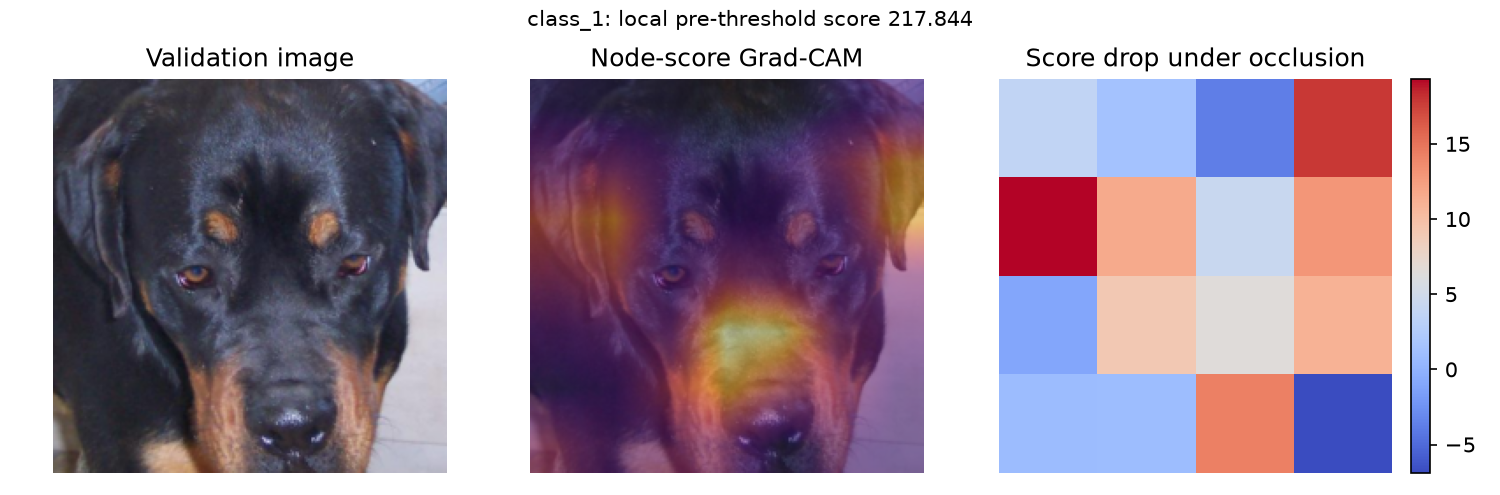
\includegraphics[width=.94\linewidth]{figures/cats_class_1.png}\\[2mm]
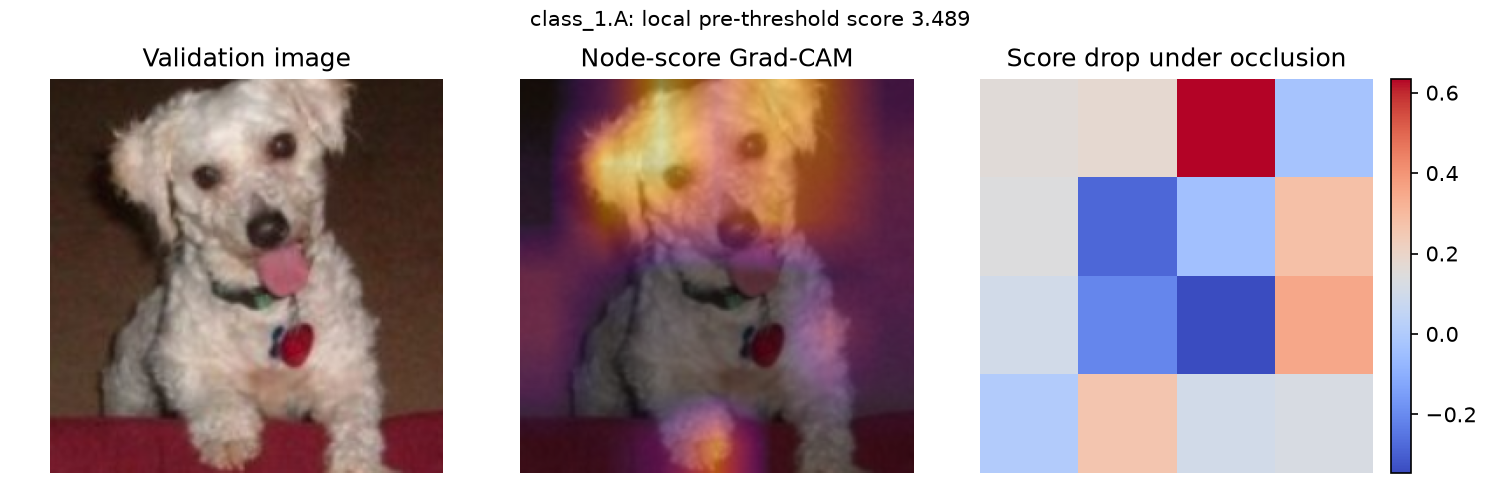
\includegraphics[width=.94\linewidth]{figures/cats_class_1_A.png}\\[2mm]
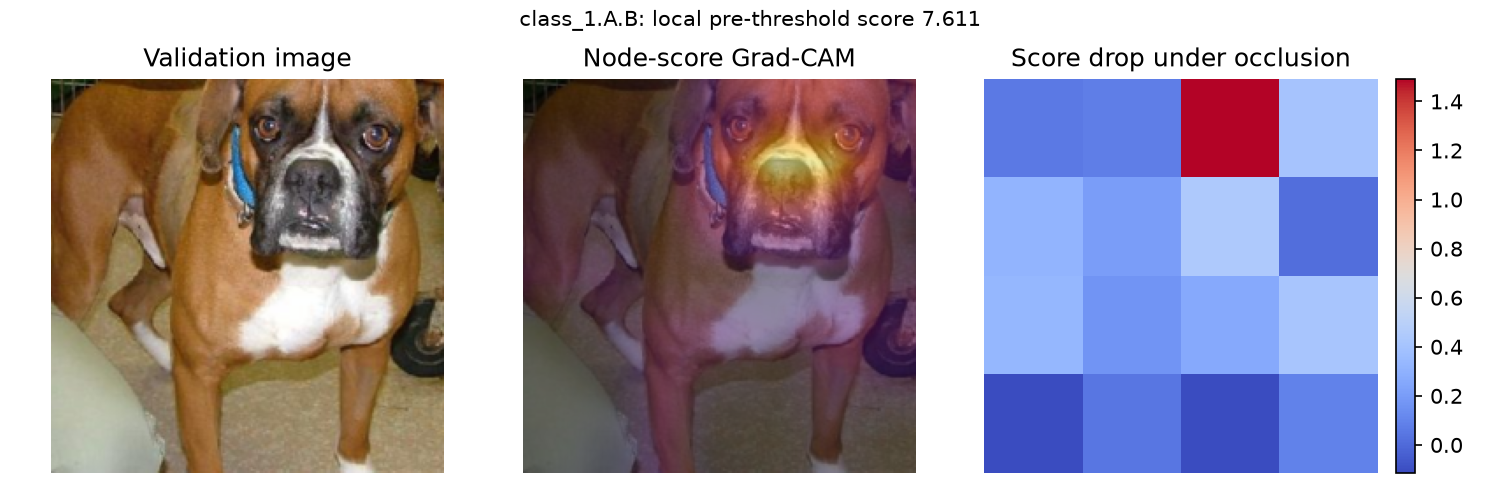
\includegraphics[width=.94\linewidth]{figures/cats_class_1_A_B.png}
\end{center}
\textbf{Figure 4.} Width-8, seed-17 unpruned tree. Rows show root $s$, child $A$, and grandchild $A.B$. Each node's highest-local-score validation example is selected independently; these are not controlled maps on the same image. The root emphasizes muzzle/ear regions; $A$ emphasizes parts of the white dog's head and surrounding boundaries. Grandchild $A.B$ emphasizes the boxer's face. Grad-CAM and occlusion overlap partly but do not agree everywhere.

$A.B$ is a negative correction for the \emph{local task of $A$}; its high activation on a dog does not mean the system has discovered a ``cat detector.'' The grandchild is subsequently pruned without loss of training fit or reported validation accuracy. Visual prominence does not imply that a node is necessary in the final composed classifier. These few top-ranked examples do not establish a general semantic specialization.

\subsection{CIFAR-10: the bird tree and a non-activating example}
\begin{center}
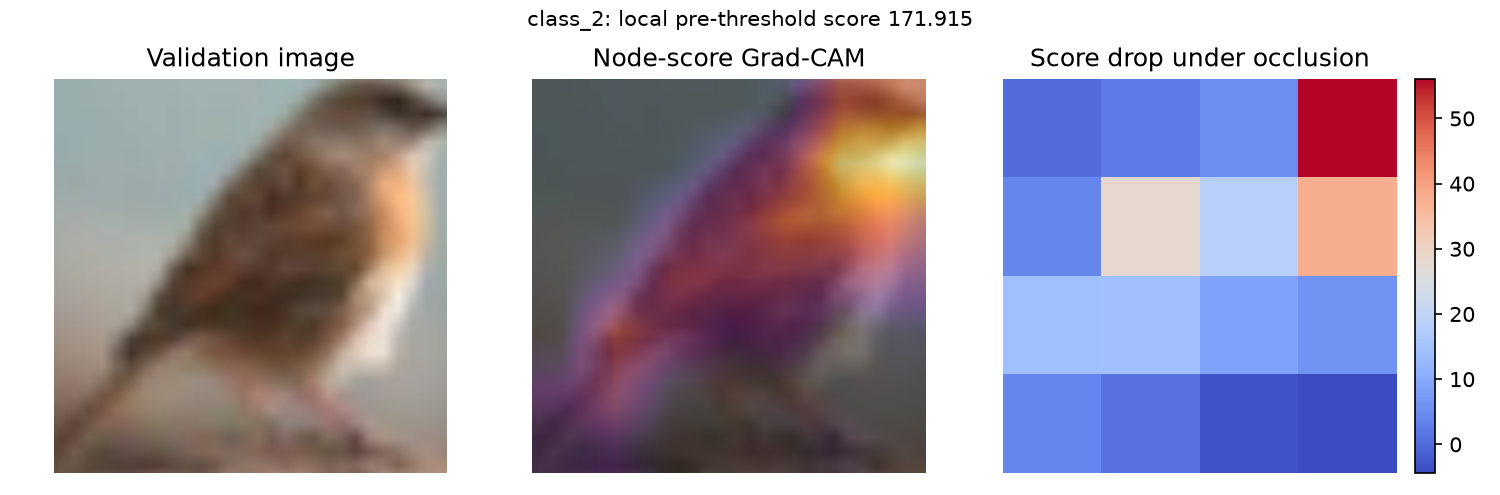
\includegraphics[width=.94\linewidth]{figures/cifar_class_2.png}\\[2mm]
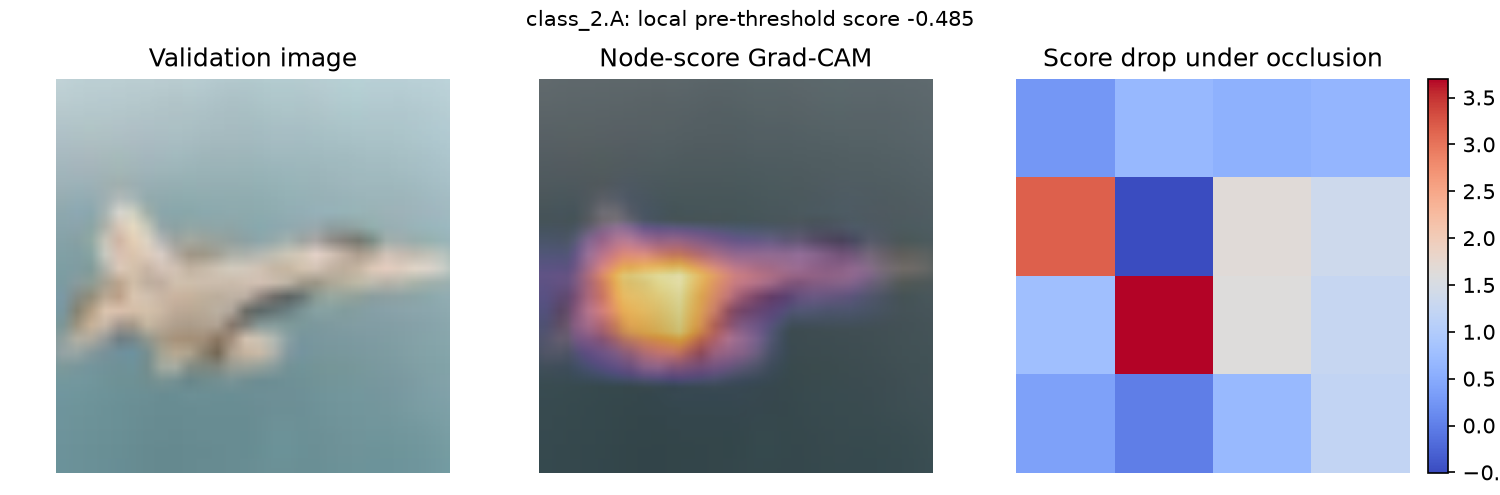
\includegraphics[width=.94\linewidth]{figures/cifar_class_2_A.png}\\[2mm]
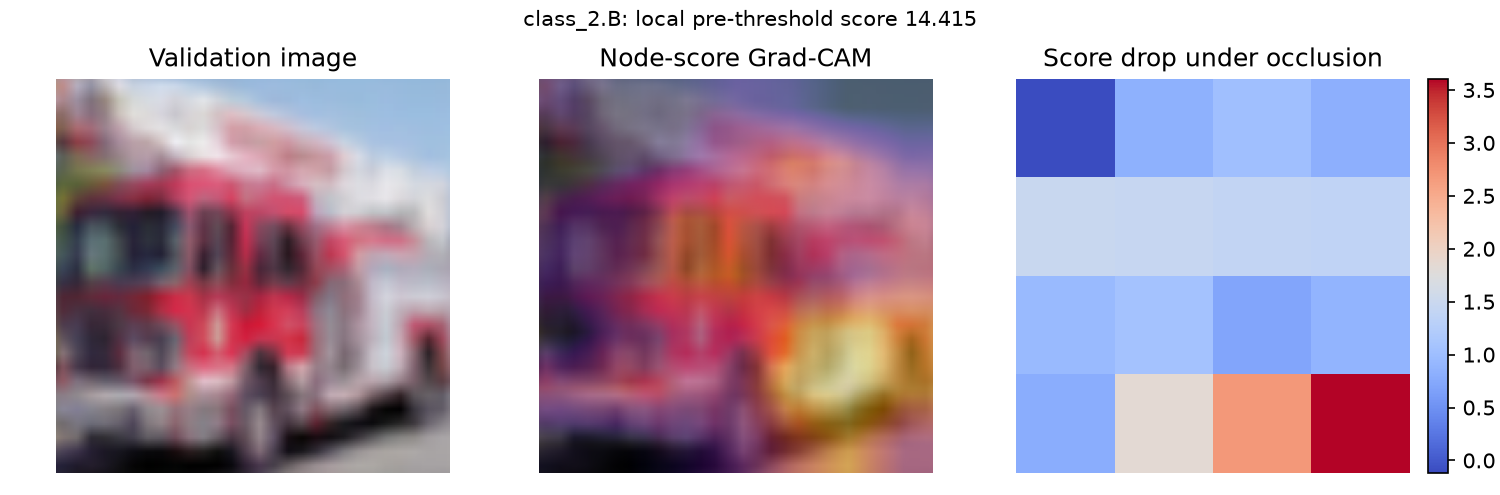
\includegraphics[width=.94\linewidth]{figures/cifar_class_2_B.png}
\end{center}
\textbf{Figure 5.} Width-16, seed-17 bird-vs-rest tree: parent, positive child $A$, and negative child $B$. The parent map emphasizes the bird's upper body/head. The $B$ example is a truck, which is compatible with learning to suppress a bird false positive, but a high local score alone does not establish that this particular validation image was actually corrected by the full tree.

The highest-ranked example shown for $A$ is an aircraft with local score $-0.485$. This leaf's decision is therefore zero on the displayed image: a bright heatmap must not be described as an active correction. The example demonstrates both the similarity of some image features and the distinction between score sensitivity and threshold activation. Enlarged $32\times32$ images and coarse feature maps limit spatial precision. Background-sensitive regions and disagreement with occlusion should temper semantic claims. The package contains all 23 node visualizations from the three prespecified seed-17 branched models, plus their high-activation examples and numeric occlusion records.

\section{Conclusions, contributions and limitations}
\textbf{What was achieved.} Neural correction nodes reach exact classification interpolation on both declared training splits, across three seeds. Pruning preserves this fit with 11--12 nodes for CIFAR-10 and two nodes for Cats vs Dogs. Root-refitting controls show that the retained corrections resolve errors left by the specified smaller-root optimization. The final test results quantify the price of enforcing perfect fit rather than assuming it improves generalization. With 15\% training-label noise, double descent appears in test error for both datasets and for the correction tree itself, with the complete classical curve on CIFAR-10; matched clean-label controls show that the noise causes the peak.

\textbf{What the tree adds.} Small nodes can distribute the task over several correction stages. Some descendants help construct a fitted model but become removable after ancestor readouts have changed. This is consistent with a training-time role for temporary branches, but the experiment is not a causal proof that those branches were the only way to learn the final weights. In the final compact models, at least one correction branch remains.

\textbf{Interpretations supported by the controls.} The final training exceptions can be expensive in parameters and confidence without improving held-out accuracy. Output refitting and interpolation substantially affect log loss even when class labels change little. Strong pretrained features make broad root-only networks sufficient at larger widths. The label-noise study explains why: corrections fit whatever the parent gets wrong, so they help when the parent's errors are genuine and hurt when its errors are mostly wrong labels. Pruning by validation accuracy, not training fit, is what turns size reduction into better generalization. On CIFAR-10, wider root-only models outperform the compact interpolating trees on test. Thus the contribution is a measured correction/compression mechanism, not a universal accuracy advantage.

\textbf{Design contributions.} The assignment combines a constrained convex readout refit, empirical error acceptance, explicit root-refit ablations, fixed-reference pruning, exact recursive prediction bounds data-provenance checks, a near-duplicate audit in feature space, and a label-noise analysis of what correction nodes learn. These are useful implementation and analysis choices, not claims of previously unpublished algorithms. Adaptive Neural Trees \cite{ant} provides a related example of learned tree structure and representations, but uses a different routing architecture; this work implements the supplied correction construction rather than reproducing that paper.

\textbf{Limits.} There are three optimization seeds on one split per dataset; the quoted SDs are not population confidence intervals. The encoder uses external supervised pretraining. Exact deduplication does not remove near-duplicates. Comparisons at equal node width do not generally match parameter count or total compute, and adaptive topology complicates double-descent claims. Pruning is greedy, interpretations use selected validation examples, and execution timing excludes feature extraction. No from-scratch trunk, joint fine-tuning, formal minimum-size solution or full calibration study is claimed. The label-noise study uses one noise rate (15\%), one noise draw for the trees and CIFAR-10, and a softmax MLP rather than one-vs-rest roots for the CIFAR-10 root-only sweep; a few runs show late training instability (Section~\ref{sec:noise}).

\section{Future directions and reproducibility}
The next useful experiments would be: (i) compare flat and branched heads at explicitly matched parameter and optimization budgets; (ii) vary the noise rate (for example 5\% and 30\%), use the tree's child-target groups to detect and relabel noisy examples, and add weight decay to remove the late training instabilities; (iii) fit calibration on a separate validation subset to distinguish confidence changes from classification changes; (iv) compress or replace the trunk, since it dominates the compact binary model; and (v) evaluate node sensitivities on matched images, including corrected and spoiled cases, rather than only top activations. A small shared trunk trained from scratch would quantify dependence on ImageNet transfer.

\paragraph{Reproducibility.} The repository linked on the first page contains the experiment code, the 14 unit tests, the run configurations, all result records under \texttt{results/}, the label-noise records under \texttt{results\_label\_noise/} (produced by \texttt{extras/run\_noise\_experiments.sh} and \texttt{extras/run\_cifar\_noise.sh}; figures and tables rebuilt by \texttt{extras/build\_noise\_report.py}), the provenance records under \texttt{provenance/}, and the LaTeX source of this report. The fixed test comparison set is recorded in \texttt{results/final\_evaluation\_protocol.json}. \texttt{README.md} gives the commands for installing the environment, regenerating the sweeps in a separate results directory (so the recorded evidence is not overwritten), and rebuilding this PDF. Image data and cached features are not stored in the repository. Trained checkpoints remain on the experiment machine; the recorded metrics, confusion matrices and prediction audits in \texttt{results/} document the reported models.

\begingroup\footnotesize
\begin{thebibliography}{9}
\setlength{\itemsep}{0pt}\setlength{\parskip}{0pt}
\bibitem{class} Jayadeva. \emph{A Tree Type Neural Network}. Supplied ELL409 class note.
\bibitem{mobilepaper} A. Howard et al. Searching for MobileNetV3. ICCV, 2019. \url{https://arxiv.org/abs/1905.02244}
\bibitem{mobile} Torchvision. MobileNetV3-Small weights and preprocessing. \href{https://docs.pytorch.org/vision/stable/models/generated/torchvision.models.mobilenet_v3_small.html}{Official model documentation}
\bibitem{cifar} A. Krizhevsky, V. Nair and G. Hinton. CIFAR-10 dataset. \href{https://www.cs.toronto.edu/~kriz/cifar.html}{Official dataset page}
\bibitem{cats} Microsoft. Kaggle Cats and Dogs Dataset, \texttt{kagglecatsanddogs\_5340.zip}. \href{https://www.microsoft.com/en-us/download/details.aspx?id=54765}{Microsoft Download Center}
\bibitem{dd} P. Nakkiran et al. Deep Double Descent: Where Bigger Models and More Data Hurt. ICLR, 2020. \url{https://arxiv.org/abs/1912.02292}
\bibitem{gradcam} R. R. Selvaraju et al. Grad-CAM: Visual Explanations from Deep Networks via Gradient-Based Localization. ICCV, 2017. \url{https://arxiv.org/abs/1610.02391}
\bibitem{ant} R. Tanno et al. Adaptive Neural Trees. ICML, 2019. \url{https://proceedings.mlr.press/v97/tanno19a.html}
\end{thebibliography}
\endgroup

\clearpage\appendix
\section{Exact final evaluation records}
\small
C10 denotes CIFAR-10 ($N_{tr}=45,000$, $N_{val}=5,000$, $N_{te}=10,000$); C/D denotes Cats vs Dogs ($17,476$, $3,745$, $3,745$). Head parameters exclude the shared 927,008-parameter encoder. Error counts prevent rounded training accuracy from concealing residual mistakes. For these original clean-label experiments, test evaluation was limited to the fixed comparison set; other clean-label sweep points remain validation-only. The label-noise study (Section~\ref{sec:noise}) selects nothing and reports test curves at every width.
\begin{longtable}{@{}lrrlrrrrr@{}}
\toprule Dataset & $h$ & Seed & Model & Head params & Train err. & Val err. & Test err. & Test (\%)\\\midrule\endhead
C10 & 16 & 17 & Root & 92,490 & 1 & 524 & 1184 & 88.16 \\
C10 & 16 & 17 & Root + refit & 92,490 & 1 & 545 & 1186 & 88.14 \\
C10 & 16 & 17 & Tree & 166,490 & 0 & 552 & 1198 & 88.02 \\
C10 & 16 & 17 & Pruned & 110,990 & 0 & 552 & 1199 & 88.01 \\
C10 & 16 & 29 & Root & 92,490 & 1 & 527 & 1153 & 88.47 \\
C10 & 16 & 29 & Root + refit & 92,490 & 1 & 531 & 1151 & 88.49 \\
C10 & 16 & 29 & Tree & 175,740 & 0 & 544 & 1181 & 88.19 \\
C10 & 16 & 29 & Pruned & 101,740 & 0 & 544 & 1181 & 88.19 \\
C10 & 16 & 43 & Root & 92,490 & 3 & 525 & 1170 & 88.30 \\
C10 & 16 & 43 & Root + refit & 92,490 & 2 & 537 & 1174 & 88.26 \\
C10 & 16 & 43 & Tree & 194,240 & 0 & 558 & 1192 & 88.08 \\
C10 & 16 & 43 & Pruned & 110,990 & 0 & 558 & 1192 & 88.08 \\
C/D & 8 & 17 & Root & 4,625 & 5 & 88 & 82 & 97.81 \\
C/D & 8 & 17 & Root + refit & 4,625 & 5 & 88 & 82 & 97.81 \\
C/D & 8 & 17 & Tree & 13,877 & 0 & 95 & 88 & 97.65 \\
C/D & 8 & 17 & Pruned & 9,251 & 0 & 95 & 88 & 97.65 \\
C/D & 8 & 29 & Root & 4,625 & 8 & 84 & 93 & 97.52 \\
C/D & 8 & 29 & Root + refit & 4,625 & 8 & 83 & 93 & 97.52 \\
C/D & 8 & 29 & Tree & 13,877 & 0 & 82 & 92 & 97.54 \\
C/D & 8 & 29 & Pruned & 9,251 & 0 & 82 & 92 & 97.54 \\
C/D & 8 & 43 & Root & 4,625 & 3 & 87 & 96 & 97.44 \\
C/D & 8 & 43 & Root + refit & 4,625 & 3 & 85 & 96 & 97.44 \\
C/D & 8 & 43 & Tree & 13,877 & 0 & 86 & 99 & 97.36 \\
C/D & 8 & 43 & Pruned & 9,251 & 0 & 86 & 99 & 97.36 \\
C/D & 16 & 17 & Root & 9,249 & 2 & 75 & 80 & 97.86 \\
C/D & 16 & 17 & Root + refit & 9,249 & 2 & 77 & 81 & 97.84 \\
C/D & 16 & 17 & Tree & 18,499 & 0 & 76 & 75 & 98.00 \\
C/D & 16 & 17 & Pruned & 18,499 & 0 & 76 & 75 & 98.00 \\
C/D & 16 & 29 & Root & 9,249 & 1 & 82 & 82 & 97.81 \\
C/D & 16 & 29 & Root + refit & 9,249 & 1 & 80 & 82 & 97.81 \\
C/D & 16 & 29 & Tree & 27,749 & 0 & 81 & 84 & 97.76 \\
C/D & 16 & 29 & Pruned & 18,499 & 0 & 81 & 84 & 97.76 \\
C/D & 16 & 43 & Root & 9,249 & 4 & 78 & 83 & 97.78 \\
C/D & 16 & 43 & Root + refit & 9,249 & 4 & 78 & 85 & 97.73 \\
C/D & 16 & 43 & Tree & 18,499 & 0 & 80 & 83 & 97.78 \\
C/D & 16 & 43 & Pruned & 18,499 & 0 & 80 & 83 & 97.78 \\
C10 & 64 & 17 & Root & 369,930 & 0 & 457 & 1003 & 89.97 \\
C10 & 64 & 17 & Root + refit & 369,930 & 0 & 461 & 1021 & 89.79 \\
C10 & 64 & 17 & Tree & 369,930 & 0 & 457 & 1003 & 89.97 \\
C10 & 64 & 17 & Pruned & 369,930 & 0 & 457 & 1003 & 89.97 \\
C10 & 256 & 17 & Root & 1,479,690 & 0 & 442 & 971 & 90.29 \\
C10 & 256 & 17 & Root + refit & 1,479,690 & 0 & 443 & 970 & 90.30 \\
C10 & 256 & 17 & Tree & 1,479,690 & 0 & 442 & 971 & 90.29 \\
C10 & 256 & 17 & Pruned & 1,479,690 & 0 & 442 & 971 & 90.29 \\
C/D & 32 & 17 & Root & 18,497 & 0 & 80 & 84 & 97.76 \\
C/D & 32 & 17 & Root + refit & 18,497 & 0 & 78 & 88 & 97.65 \\
C/D & 32 & 17 & Tree & 18,497 & 0 & 80 & 84 & 97.76 \\
C/D & 32 & 17 & Pruned & 18,497 & 0 & 80 & 84 & 97.76 \\
\bottomrule

\end{longtable}
\end{document}

